\chapter{Wahrscheinlichkeit, Information und Entropie}

\lectureoverview{Die statistische Mechanik beginnt dort, wo mikroskopische Gesetze auf unvollständiges Wissen treffen. Zunächst präzisieren wir den Wahrscheinlichkeitsbegriff. Dann fragen wir, wie die deterministische Bewegung selbst Wahrscheinlichkeiten festlegt, wie Erhaltungssätze den Zustandsraum aufteilen und warum informationsbewahrende Dynamik ganz natürlich zur Entropie führt. Der erste und der nullte Hauptsatz kommen erst ins Spiel, wenn diese Struktur steht.}

\section{Warum statistische Mechanik?}

Die statistische Mechanik wird manchmal als alte Physik bezeichnet. Das verfehlt den entscheidenden Punkt. Sie ist vormodern, modern und wird wohl auch in jeder postmodernen Physik nützlich bleiben, die auf die uns bekannten Theorien folgt. Einzelne Modelle kommen und gehen; der zweite Hauptsatz der Thermodynamik hat sich wiederholt als verlässlicher Wegweiser erwiesen. Wann immer eine vorgeschlagene Beschreibung der Natur scheinbar kostenlos Ordnung erzeugt, Information grundlegend auslöscht oder ein abgeschlossenes System in einen unnatürlich einfachen Zustand überführt, warnt uns der zweite Hauptsatz, dass etwas fehlt.

Das Fach mag weniger glamourös erscheinen als ein neu entdecktes Teilchen, ist aber mindestens ebenso tiefgründig und wesentlich allgemeiner. Gase, Flüssigkeiten, Festkörper, Strahlung, Schwarze Löcher, Information und Quantenfelder erfordern statistisches Denken. Tatsächlich ließe sich die experimentelle Technik, mit der Teilchen entdeckt werden, ohne dieses Denken gar nicht verstehen. Deshalb haben Generationen herausragender Physikerinnen und Physiker die statistische Mechanik gemeistert, auch wenn ihr Hauptarbeitsgebiet anderswo lag: Das Fach ist nützlich, aber auch ungewöhnlich schön.

Um zu sehen, warum sie gebraucht wird, beginnen wir mit dem Ideal der Mechanik. Ein abgeschlossenes System ist entweder das gesamte betrachtete Universum oder ein Teilsystem, das so gut isoliert ist, dass seine Umgebung es nicht beeinflusst. Kennen wir seinen Anfangszustand und sein Entwicklungsgesetz, ermöglicht die klassische Mechanik eine vollständige Vorhersage. Die Quantenmechanik schränkt ein, was sich vorhersagen lässt; doch auch sie hat einen genau definierten Zustand und ein Gesetz, das die maximal mögliche Information vorhersagt, die die Theorie zulässt.

Zwischen Vorhersagbarkeit im Prinzip und brauchbarem Verständnis besteht ein erheblicher Unterschied. Eine Liste der Positionen und Geschwindigkeiten aller Moleküle in diesem Raum wäre unfassbar lang, würde sich fast sofort ändern und nur wenige der Fragen beantworten, die uns tatsächlich interessieren. Exakte mikroskopische Gesetze können also zugleich vollkommen vorhersagekräftig und praktisch nutzlos sein.

Die statistische Mechanik ist die auf diese physikalische Situation angewandte Wahrscheinlichkeitstheorie. Sie wird nötig, wenn der Anfangszustand nicht mit vollkommener Genauigkeit bekannt ist, das Gesetz nur näherungsweise bekannt ist, das System offen ist oder schlicht zu viele mikroskopische Variablen vorliegen, um sie zu verfolgen. Das bedeutet keineswegs, dass die Vorhersagen ungenau sein müssen. Bei großen Zahlen können statistische Vorhersagen außerordentlich präzise sein.

Betrachten wir einen isolierten Gaskasten. Wir können die Bahn jedes einzelnen Moleküls nicht vorhersagen, aber aus wenigen makroskopischen Angaben lassen sich Druck, Energie und viele weitere makroskopische Größen mit hoher Genauigkeit vorhersagen. Ungewiss bleiben die Fluktuationen. Zu einem unvorhersehbaren Zeitpunkt kann ein kleines Gebiet mehr Moleküle als im Mittel enthalten, während ein anderes weniger enthält. Ein solches Ereignis liegt im Randbereich einer Wahrscheinlichkeitsverteilung: Es ist unwahrscheinlich, aber nicht ausgeschlossen. Wir können berechnen, wie oft solche Fluktuationen auftreten sollten, ohne den Zeitpunkt eines einzelnen Ereignisses vorherzusagen.

Beim Münzwurf zeigt sich derselbe Unterschied. Bei einer Milliarde fairer Würfe werden Kopf und Zahl annähernd gleich häufig auftreten. Bei genügend vielen Würfen wird irgendwann eine lange Folge von Kopf auftreten; die Wahrscheinlichkeitstheorie sagt jedoch deren Häufigkeit voraus, nicht, wann sie eintreten wird. Die statistische Mechanik ist für Systeme gedacht, deren Bestandteile zu klein, zu zahlreich oder beides sind.

Im Kurs entwickeln wir die Gesetze ebenso wie ihre Anwendung auf Materie. Das Fach lohnt wiederholtes Lernen: Man lernt es, vergisst Teile davon und lernt es erneut, mit einem tieferen Verständnis dafür, welche Ideen grundlegend sind. Wir beginnen mit dem Begriff, der alles Weitere bestimmt.

\section{Wahrscheinlichkeit als grundlegende Sprache}

Warum Wahrscheinlichkeit funktioniert, erklärt die Wahrscheinlichkeitsrechnung selbst nicht. Eine probabilistische Vorhersage kann bei einem einzelnen Versuch scheitern; genau das bedeutet es, dass ein Ergebnis möglich, aber unwahrscheinlich ist. Die Theorie sagt uns, wie die Ausnahmen verteilt sind. Sie schafft sie nicht ab. Wir nehmen Wahrscheinlichkeit daher als Grundbegriff und formulieren die Regeln, denen sie genügt.

\subsection{Zustände und Normierung}

Sei \(i\) die Bezeichnung für ein mögliches Ergebnis oder einen möglichen Zustand eines Systems. Bei einer Münze kann \(i\) für Kopf oder Zahl stehen. Bei einem Würfel kann \(1\) bis \(6\) durchlaufen. Bei zwei Würfeln hält ein Indexpaar beide Augenzahlen fest. Zunächst betrachten wir einen endlichen diskreten Zustandsraum,
\begin{equation}
 i=1,\ldots,N,
\end{equation}
und gehen später zu unendlich vielen und kontinuierlich vielen Zuständen über.

Unwissenheit bedeutet nicht, dass das System keinen Zustand hat. Sie bedeutet, dass wir nicht wissen, welchen Zustand es hat, und deshalb jeder Möglichkeit eine Wahrscheinlichkeit \(p_i\) zuweisen. Die Grundregeln lauten
\begin{align}
 p_i &\geq 0, \label{eq:sm1-prob-positive}\\
 \sum_{i=1}^{N}p_i &=1. \label{eq:sm1-prob-normalization}
\end{align}
Die Alternativen schließen einander aus und sind vollständig: Genau eine von ihnen tritt ein. Negative Wahrscheinlichkeiten spielen hier keine Rolle, und die Summe ist eins, weil eines der zulässigen Ergebnisse eintreten muss.

\subsection{Häufigkeit und Gesetz der großen Zahlen}

Wahrscheinlichkeit ist durch wiederholte Versuche mit dem Experiment verknüpft. Angenommen, dasselbe Experiment wird \(N_{\mathrm{trials}}\) Mal durchgeführt, und \(N(i)\) sei die Anzahl der Versuche, bei denen das Ergebnis \(i\) auftritt. Dann lautet die Häufigkeitsdeutung
\begin{equation}
 p_i=
 \lim_{N_{\mathrm{trials}}\to\infty}
 \frac{N(i)}{N_{\mathrm{trials}}}.
 \label{eq:sm1-frequency}
\end{equation}
Dies ist eine physikalische Hypothese, ausgedrückt durch einen idealisierten Grenzwert. Kein Labor führt unendlich viele Experimente durch. Die Aussage ist, dass bei genügend vielen Versuchen das Verhältnis nahe genug an \(p_i\) heranrückt, um die beabsichtigte Vorhersage zu ermöglichen. Endliche Stichproben fluktuieren um den Grenzwert.

\subsection{Mittelwerte}

Ordnen wir nun jedem Zustand eine Zahl \(f(i)\) zu. Sie kann die Energie, der Impuls oder eine andere Größe sein, die wir messen möchten. Ihr Erwartungswert ist
\begin{equation}
 \langle f\rangle=\sum_i f(i)p_i.
 \label{eq:sm1-expectation}
\end{equation}
Die Klammernotation ist auch außerhalb der Quantenmechanik praktisch. In der Sprache der Häufigkeiten lautet derselbe Mittelwert
\begin{equation}
 \langle f\rangle
 =
 \lim_{N_{\mathrm{trials}}\to\infty}
 \frac{1}{N_{\mathrm{trials}}}
 \sum_i f(i)N(i).
 \label{eq:sm1-frequency-average}
\end{equation}

Für eine Münze definieren wir
\begin{equation}
 f(\mathrm{H})=+1,
 \qquad
 f(\mathrm{T})=-1.
\end{equation}
Wenn Kopf und Zahl jeweils die Wahrscheinlichkeit \(1/2\) haben, gilt
\begin{equation}
 \langle f\rangle
 =(+1)\frac12+(-1)\frac12=0.
\end{equation}
Der Mittelwert muss kein mögliches Ergebnis sein. Die Münze landet nie auf null; null fasst die Verteilung ihrer beiden möglichen Werte zusammen.

Dieser kurze Einschub legt die Begriffe fest, die im gesamten Fach verwendet werden: Zustände, Wahrscheinlichkeiten, Häufigkeiten und Erwartungswerte.

\section{Drei Wege, Wahrscheinlichkeiten zuzuweisen}

\subsection{Symmetrie}

Warum weisen wir den beiden Münzseiten gewöhnlich gleiche Wahrscheinlichkeiten zu? Die erste Antwort lautet: Symmetrie. Das Wenden einer annähernd idealen Münze vertauscht Kopf und Zahl, ohne das Experiment zu verändern. Es gibt dann keinen physikalischen Grund, ein Ergebnis zu bevorzugen. Eine echte Markierung oder Unregelmäßigkeit führt zu einer winzigen Verzerrung, doch das symmetrische Modell beschreibt das beabsichtigte Experiment:
\begin{equation}
 p(\mathrm{H})=p(\mathrm{T})=\frac12.
\end{equation}

Dasselbe Argument weist jeder Seite eines symmetrischen Würfels die Wahrscheinlichkeit \(1/6\) zu. Allgemeiner gilt: Konfigurationen, die durch eine Symmetrie ineinander überführt werden, erhalten gleiche Wahrscheinlichkeiten, sofern keine zusätzlichen Informationen diese Symmetrie brechen.

\subsection{Experiment}

Ein unregelmäßig geformter Würfel hat keine Symmetrie, die alle sechs Seiten vertauscht. In diesem Fall liefert die Symmetrie allein keine Antwort. Vielleicht besitzt man ein tiefergehendes mechanisches Modell, das die Verzerrung vorhersagt. Ohne ein solches Modell ist das ehrliche Vorgehen jedoch experimentell: Man wirft den Würfel viele Male, erfasst die Häufigkeiten, wartet, bis sie sich stabilisieren, und verwendet die so gewonnene Wahrscheinlichkeitstabelle für spätere Vorhersagen.

Symmetrie und Experiment sind keine konkurrierenden Definitionen. Sie sind zwei Quellen für Informationen über eine Wahrscheinlichkeitsverteilung. Die statistische Mechanik stützt sich stark auf Symmetrie, doch die Dynamik bietet einen dritten Weg.

\subsection{Wahrscheinlichkeit aus deterministischer Bewegung}

Stellen wir uns einen unregelmäßigen Gegenstand mit sechs farbigen Konfigurationen vor. In festen diskreten Zeitabständen wechselt er gemäß einem eindeutigen Aktualisierungsgesetz seinen Zustand:
\begin{equation}
 R\longrightarrow B\longrightarrow Y\longrightarrow G
 \longrightarrow O\longrightarrow P\longrightarrow R.
 \label{eq:sm1-six-cycle}
\end{equation}
Der Gegenstand selbst muss keine geometrische Symmetrie besitzen. Das Gesetz legt lediglich fest, welche Konfiguration auf eine gegebene folgt.

\begin{figure}[htbp]\centering
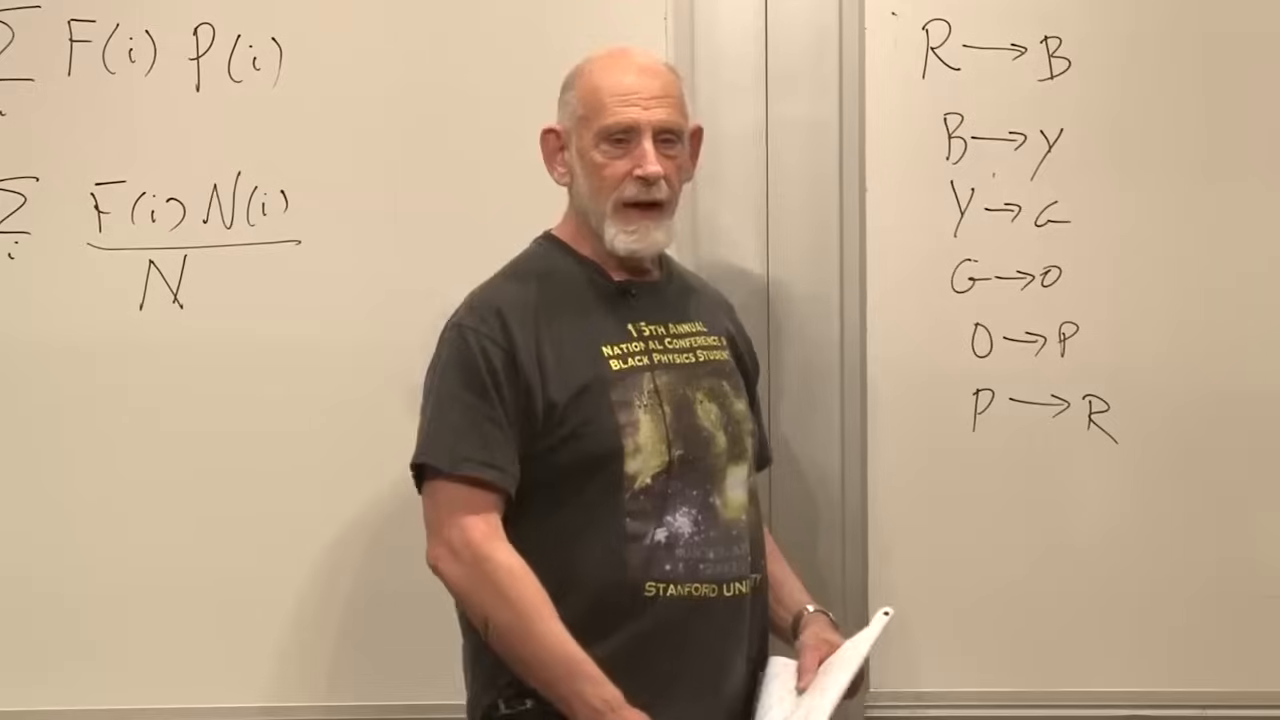
\includegraphics[width=0.92\textwidth]{lecture_01_figure_02.png}\caption{Die Erwartungswertformeln bleiben auf der linken Tafel stehen, während rechts die sechs deterministischen Farbwechsel aufgeführt sind.}\lectureframe{00:26:28}\end{figure}

Übersichtlicher lässt sich die Tafel als gerichteter Zyklus darstellen:
\begin{figure}[htbp]\centering
\begin{tikzpicture}[
  >=Latex,
  state/.style={draw,circle,minimum size=8mm,inner sep=1pt}
]
\node[state] (R) at (90:2.2) {$R$};
\node[state] (B) at (30:2.2) {$B$};
\node[state] (Y) at (-30:2.2) {$Y$};
\node[state] (G) at (-90:2.2) {$G$};
\node[state] (O) at (-150:2.2) {$O$};
\node[state] (P) at (150:2.2) {$P$};
\draw[->] (R) -- (B);
\draw[->] (B) -- (Y);
\draw[->] (Y) -- (G);
\draw[->] (G) -- (O);
\draw[->] (O) -- (P);
\draw[->] (P) -- (R);
\end{tikzpicture}\caption{Ein einzelner Orbit mit sechs Zuständen. Während jeder Periode wird jeder Zustand einmal durchlaufen.}\label{fig:sm1-six-cycle}\end{figure}

Angenommen, wir kennen den Anfangszustand nicht und machen zu einem unbekannten Zeitpunkt eine Momentaufnahme. Da jeder Schritt gleich lange dauert, verbringt das System ein Sechstel einer Periode in jeder Farbe:
\begin{equation}
 p(R)=p(B)=p(Y)=p(G)=p(O)=p(P)=\frac16.
 \label{eq:sm1-uniform-cycle}
\end{equation}
Die Gleichheit folgt nicht aus der Form des Gegenstands. Sie ergibt sich daraus, dass das System gleich lange in den einzelnen Zuständen verweilt.

Wir können die Pfeile neu anordnen und so ein anderes mikroskopisches Gesetz erhalten, das weiterhin einen Zyklus mit sechs Zuständen bildet. Die genaue Abfolge ändert sich, doch die Wahrscheinlichkeit für eine Momentaufnahme bleibt \(1/6\), weil jeder Zustand weiterhin einmal pro Periode auftritt. Für diese Vorhersage brauchen wir daher weder den Startpunkt noch die genaue Reihenfolge. Es genügen die Orbitstruktur und eine gleiche Verweildauer pro Schritt.

\begin{classroomqa}\classquestion{Wenn der Gegenstand nicht symmetrisch ist, in welchem Sinn ist es dann zulässig, jeder Farbe die Wahrscheinlichkeit \(1/6\) zuzuweisen?}\lecturerresponse{Die Zuweisung ist dynamischer, nicht geometrischer Art. Eine Momentaufnahme zu einer unbekannten Phase eines Zyklus mit sechs Schritten erfasst einen von sechs gleich langen Zeitabschnitten. Gleichwertig sind dabei die Positionen auf dem Orbit, nicht die Seiten des Gegenstands. Bei ungleichen Verweildauern wären auch die Wahrscheinlichkeiten ungleich.
\lecturetimestamp{00:27:11--00:29:49}}\end{classroomqa}

\section{Getrennte Zyklen und Erhaltungsgrößen}

Ein deterministisches Gesetz muss nicht alle Zustände auf einen einzigen Orbit legen. Betrachten wir zwei getrennte Zyklen,
\begin{equation}
 R\longrightarrow B\longrightarrow G\longrightarrow R,
 \qquad
 P\longrightarrow Y\longrightarrow O\longrightarrow P.
 \label{eq:sm1-two-cycles}
\end{equation}
Wissen wir, dass das System auf dem ersten Zyklus liegt, gilt
\begin{equation}
 \begin{aligned}
 p(R)=p(B)=p(G)&=\frac13,\\
 p(P)=p(Y)=p(O)&=0.
 \end{aligned}
\end{equation}
Wissen, dass es auf dem zweiten Zyklus liegt, vertauscht diese Zuordnungen.

Im allgemeineren Fall braucht man vorgegebene Gewichte. Bezeichnen wir die Zyklen mit \(+1\) und \(-1\) und ihre Wahrscheinlichkeiten mit \(p_+\) und \(p_-\), wobei
\begin{equation}
 p_++p_-=1.
\end{equation}
Dann gilt
\begin{align}
 p(R)=p(B)=p(G)&=\frac{p_+}{3},\\
 p(P)=p(Y)=p(O)&=\frac{p_-}{3}.
 \label{eq:sm1-sector-weights}
\end{align}
Die Faktoren \(1/3\) folgen aus der Bewegung innerhalb eines Zyklus. Die Zahlen \(p_+\) und \(p_-\) tun das nicht. Sie müssen aus zusätzlichen Informationen stammen, vielleicht aus einem weiteren Experiment oder einem anderen System, das den Anfangssektor auswählt.

Die Bezeichnungen \(+1\) und \(-1\) definieren eine Erhaltungsgröße: Beginnt das System auf einem Zyklus, führt das Aktualisierungsgesetz es niemals auf den anderen. Man kann die Größe Energie nennen oder ihr einen Platzhalternamen wie \emph{Nullgröße} geben. Ihr Name ist zweitrangig. Erhaltung bedeutet, dass der Zustandsraum in Bereiche aufgeteilt ist, die die Dynamik nicht überschreiten kann.

Die Zyklen müssen nicht gleich viele Zustände enthalten. Auch ein Orbit mit vier Zuständen und einer mit zwei Zuständen bilden zwei erhaltene Sektoren. Die Gleichzeitstichprobe ergibt dann innerhalb des ersten \(1/4\) und innerhalb des zweiten \(1/2\), jeweils multipliziert mit der vorgegebenen Wahrscheinlichkeit des betreffenden Sektors. Die statistische Mechanik muss zwei logisch getrennte Fragen beantworten:
\begin{enumerate}\item Wie viel Zeit verbringt die Dynamik, gegeben einen erhaltenen Sektor, in dessen Zuständen?
\item Welche Wahrscheinlichkeit ist dem erhaltenen Sektor selbst zuzuweisen?
\end{enumerate}

\begin{classroomqa}\audiencequestion{Nehmen wir an, dass alle Zustände innerhalb eines erhaltenen Sektors dieselbe Wahrscheinlichkeit erhalten?}\lecturerresponse{Für die hier gezeigten diskreten Spielzeuggesetze: ja, denn jeder Zustand dauert gleich lang und die Bewegung ist deterministisch. Unbekannt ist die Anfangsphase des Orbits. Ein Detektor mit Millisekunden-Auflösung kann Aktualisierungen im Mikrosekundenbereich nicht auflösen, doch eine hinreichend schnelle Momentaufnahme kann den erfassten Zustand weiterhin bestimmen. In einem allgemeineren System müssen ungleiche Verweildauern ausdrücklich berücksichtigt werden.
\lecturetimestamp{00:36:16--00:37:17}}\end{classroomqa}

\begin{classroomqa}\audiencequestion{Wenn zwei Momentaufnahmen gemacht werden und die erste einen Zyklus identifiziert, sollte die zweite dann denselben Zyklus identifizieren?}\lecturerresponse{Ja. Genau das bedeutet Erhaltung. Sobald eine Messung den Wert der Erhaltungsgröße bestimmt, können künftige Wahrscheinlichkeiten auf diesen Wert bedingt werden; Zustände im anderen Sektor erhalten dann die Wahrscheinlichkeit null.
\lecturetimestamp{00:37:18--00:37:45}}\end{classroomqa}

\subsection{Zwischen zwei Systemen geteilte Energie}

Ersetzen wir nun die abstrakte Bezeichnung durch Energie. Ein einzelner isolierter Kasten ist ein abgeschlossenes System und hat eine erhaltene Energie. Zwei isolierte Kästen haben zwei jeweils getrennt erhaltene Energien, weil sie nicht miteinander wechselwirken. Verbindet man sie durch einen schmalen Durchgang, durch den Energie fließen kann, können sich die einzelnen Energien ändern, während die Gesamtenergie erhalten bleibt.

\begin{figure}[htbp]\centering
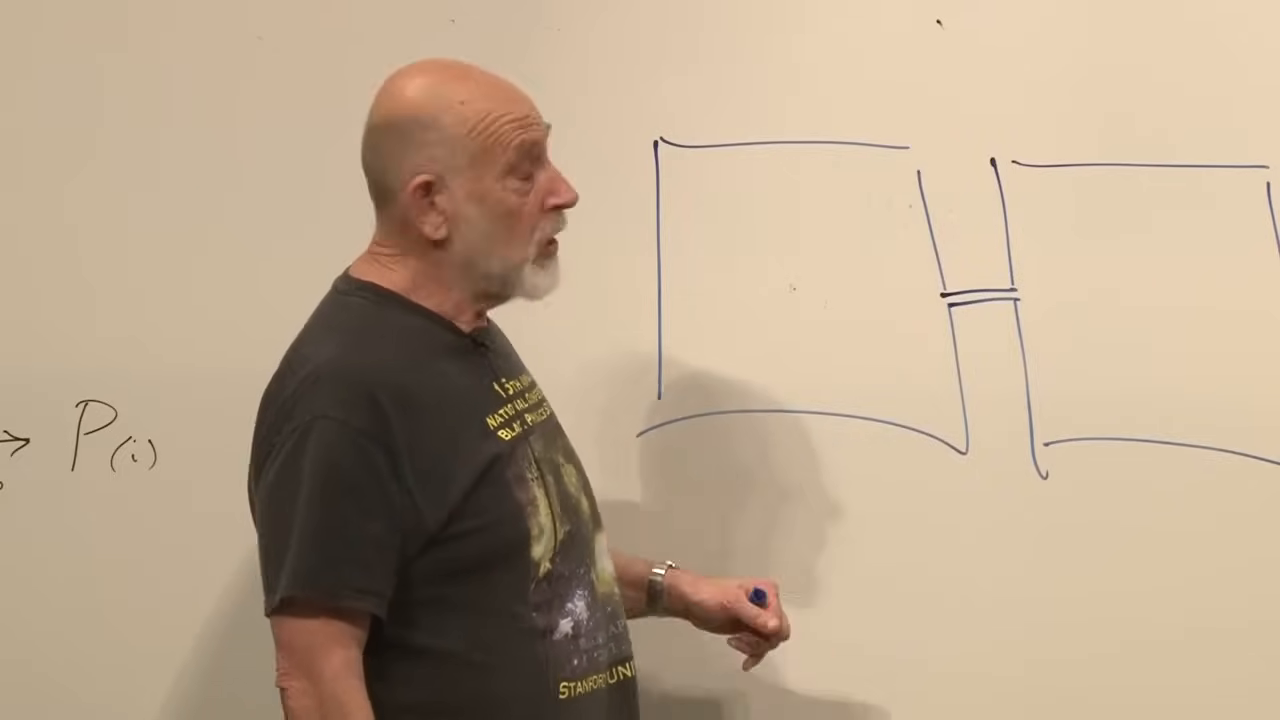
\includegraphics[width=0.92\textwidth]{lecture_01_figure_03.png}\caption{Zwei Teilsysteme, verbunden durch einen schmalen Kanal, durch den Energie fließen kann.}\lectureframe{00:39:19}\end{figure}

\begin{figure}[htbp]\centering
\begin{tikzpicture}[>=Latex]
\draw[thick,rounded corners=4pt] (-4,1.8) rectangle (-0.7,-1.5);
\draw[thick,rounded corners=4pt] (0.7,1.5) rectangle (4,-1.8);
\draw[thick] (-0.7,0.45) -- (0.7,0.45);
\draw[thick] (-0.7,-0.35) -- (0.7,-0.35);
\draw[<->,very thick] (-0.45,0.05) -- (0.45,0.05);
\node at (-2.35,0.15) {subsystem \(1\)};
\node at (2.35,-0.15) {subsystem \(2\)};
\node[above] at (0,0.5) {energy exchange};
\end{tikzpicture}\caption{Nach dem Öffnen der Verbindung ist nur noch \(E_1+E_2\) erhalten. Die Energieaufteilung wird zu einem Wahrscheinlichkeitsproblem.}\label{fig:sm1-connected-systems}\end{figure}

Bei gegebener Gesamtenergie können wir nach der Wahrscheinlichkeit fragen, dass Teilsystem \(1\) die Energie \(E_1\) hat, während Teilsystem \(2\) den Rest besitzt. Im Mittel sollten gleich große Kästen gleich viel Energie haben, doch der Mittelwert beschreibt nicht die gesamte Verteilung. Eine Möglichkeit, Wahrscheinlichkeiten für ein Teilsystem zu bestimmen, besteht daher darin, es in ein größeres abgeschlossenes System einzubetten, dessen Erhaltungssatz die fehlenden Informationen liefert. Diese Konstruktion wird in der statistischen Mechanik immer wieder auftauchen.

\section{Gute Gesetze, schlechte Gesetze und der minus erste Hauptsatz}

Nicht jede deterministische Aktualisierungsregel ist als fundamentales Gesetz zulässig. Betrachten wir die Abbildung
\begin{equation}
 \begin{aligned}
 R&\mapsto R,& B&\mapsto R,& Y&\mapsto R,\\
 G&\mapsto R,& O&\mapsto R,& P&\mapsto R.
 \end{aligned}
 \label{eq:sm1-all-to-red}
\end{equation}
Sie sagt die Zukunft perfekt voraus: Nach einem Schritt ist der Zustand rot. In umgekehrter Richtung versagt sie. Ist das System einmal rot, lässt sich nicht erkennen, ob es zuvor blau, gelb, grün, orange, violett oder ebenfalls rot war.

\begin{figure}[htbp]\centering
\begin{tikzpicture}[
  >=Latex,
  state/.style={draw,circle,minimum size=8mm,inner sep=1pt}
]
\node[state,fill=red!12] (R) at (0,0) {$R$};
\node[state] (B) at (-3,1.6) {$B$};
\node[state] (Y) at (-3,0) {$Y$};
\node[state] (G) at (-3,-1.6) {$G$};
\node[state] (O) at (3,1.6) {$O$};
\node[state] (P) at (3,-1.6) {$P$};
\draw[->] (B) -- (R);
\draw[->] (Y) -- (R);
\draw[->] (G) -- (R);
\draw[->] (O) -- (R);
\draw[->] (P) -- (R);
\draw[->,loop above] (R) to (R);
\end{tikzpicture}\caption{Ein Gesetz, das viele Zustände auf einen abbildet, sagt den nächsten Zustand voraus, löscht aber die Unterscheidungen zwischen möglichen früheren Zuständen aus.}\label{fig:sm1-bad-law}\end{figure}

Ein geschlossener Zyklus bewahrt dagegen die Aufzeichnung. Ist die verstrichene Zeit bekannt, können wir den Zustand vorwärts oder rückwärts entwickeln, selbst nach vielen Tausend Perioden. Das Gesetz erhält die Unterscheidbarkeit der Anfangsbedingungen. Susskind nennt diese Forderung den \emph{minus ersten Hauptsatz der Physik}: Information geht nicht grundlegend verloren.

Für einen endlichen diskreten Zustandsraum ist das Kriterium im Diagramm einfach:
\begin{quote}
Von jedem Zustand eines guten Gesetzes geht genau ein Pfeil aus, und genau ein Pfeil führt in ihn hinein.
\end{quote}
Der ausgehende Pfeil bestimmt die Zukunft; der eingehende rekonstruiert die Vergangenheit. Mathematisch ist die Aktualisierung eine Permutation der Zustände.

\subsection{Reibung ist nur ein scheinbares Gegenbeispiel}

Das kontinuierliche Gegenstück ist der Satz von Liouville. Reibung scheint ihm zu widersprechen. Schiebt man einen Radiergummi über einen Tisch, kommt er unabhängig davon, wo er startet, schließlich zur Ruhe. Eine schematische Gleichung für den Widerstand lautet
\begin{equation}
 m\ddot x=-\gamma\dot x,
 \qquad \gamma>0.
 \label{eq:sm1-drag}
\end{equation}
Seine Geschwindigkeit nimmt exponentiell ab. Wäre dies das fundamentalste Gesetz für jedes Teilchen in einem versiegelten Raum, käme alle Bewegung zum Erliegen, die Temperatur sänke auf null, und viele Anfangszustände würden zu einem einzigen Endzustand zusammenfallen. Die Energieerhaltung wäre verletzt, Information ginge verloren und die Unordnung nähme ab. Das wäre im Kontinuum das Gegenstück dazu, dass alles rot wird.

Echte Reibung bewirkt das nicht. Der Radiergummi erwärmt den Tisch, sich selbst und die Umgebung. Mikroskopische Positionen und Impulse halten die Unterscheidungen fest, die in der sichtbaren Bewegung verloren gehen. Reibung ist eine effektive Gleichung für ein Teilsystem, nachdem unbeobachtete Freiheitsgrade ausgeblendet wurden; sie ist kein fundamentales dissipatives Gesetz für das vollständige abgeschlossene System.

\begin{classroomqa}\classquestion{Was beschreibt die Differentialgleichung \(m\ddot x=-\gamma\dot x\), und warum ist sie kein fundamentales Gesetz für ein abgeschlossenes System?}\lecturerresponse{Sie beschreibt viskosen Widerstand. Für sich genommen treibt sie jede Geschwindigkeit gegen null; damit würde ein Gas unabhängig von seiner Anfangstemperatur auf null abkühlen. In einer tatsächlichen Beschreibung eines abgeschlossenen Systems gehen die verlorene mechanische Energie und Information in mikroskopische Freiheitsgrade über. Die Widerstandsgleichung ist nur dann verlässlich, wenn diese Variablen unterdrückt wurden.
\lecturetimestamp{00:44:40--00:48:56}}\end{classroomqa}

\section{Besetzte Zustände und die erste Entropie}

Die Erhaltung der Information hat eine entsprechende probabilistische Aussage. Angenommen, \(M\) von \(N\) Zuständen wird jeweils dieselbe Wahrscheinlichkeit zugewiesen:
\begin{equation}
 p_i=
 \begin{cases}
 1/M, & i\text{ in the occupied set},\\
 0, & i\text{ outside it}.
 \end{cases}
 \label{eq:sm1-uniform-occupied}
\end{equation}
Eine informationsbewahrende Aktualisierung kann die besetzten Zustände neu verteilen, aber sie kann sie nicht zusammenführen. Zu jedem späteren Zeitpunkt gibt es weiterhin \(M\) Zustände mit der Wahrscheinlichkeit \(1/M\). Die schlechte Abbildung \eqref{eq:sm1-all-to-red} kann dagegen viele besetzte Zustände zu einem einzigen zusammenfallen lassen.

Die Zahl \(M\) misst Unwissenheit. Wenn \(M=N\) gilt, ist jeder Zustand möglich und unsere Unwissenheit maximal. Wenn \(M=1\) gilt, ist der mikroskopische Zustand genau bekannt. Die erste Definition der Entropie lautet daher
\begin{equation}
 S=\log M.
 \label{eq:sm1-entropy-logm}
\end{equation}
Damit ergibt sich
\begin{equation}
 S_{\max}=\log N,
 \qquad
 S_{\min}=0.
\end{equation}
Ist der Zustandsraum unendlich, muss es keine endliche obere Schranke geben.

In dieser Darstellung tritt die Entropie vor der Temperatur auf, sogar vor der formalen Formulierung der Energieerhaltung. In diesem Sinn ist sie grundlegender. Sie ist jedoch keine Eigenschaft des mechanischen Systems allein. Sie hängt sowohl vom System als auch von der Wahrscheinlichkeitsverteilung ab, die das bekannte Wissen repräsentiert. Verschiedene Beobachter mit unterschiedlichem Wissen können demselben mechanischen System unterschiedliche Entropien zuweisen.

Bei exakter mikroskopischer Entwicklung werden die besetzten Zustände lediglich neu angeordnet; diese feinkörnige Entropie bleibt also erhalten. In der Praxis verlieren wir die zeitliche Auflösung, verwerfen Korrelationen und können die enorm vielen Variablen nicht verfolgen. Unsere Wahrscheinlichkeitsverteilung erstreckt sich dann über mehr Alternativen, und die der grobkörnigen Beschreibung zugewiesene Entropie nimmt zu. Die Gleichungen müssen Information nicht zerstören, damit unsere brauchbare Beschreibung sie verliert.

\begin{classroomqa}\classquestion{Wie groß ist die maximal mögliche Entropie eines endlichen Systems mit \(N\) Zuständen?}\lecturerresponse{Sie beträgt \(\log N\) und wird erreicht, wenn alle \(N\) Zustände gleich wahrscheinlich sind. Die minimale Entropie ist null und wird erreicht, wenn ein Zustand die Wahrscheinlichkeit eins hat. Entropie misst somit sowohl den Wissensstand als auch den verfügbaren Zustandsraum.
\lecturetimestamp{00:56:46--00:58:19}}\end{classroomqa}

\section{Liouville-Fluss im kontinuierlichen Phasenraum}

Bei Teilchen mit kontinuierlichen Positionen und Impulsen entspricht ein mikroskopischer Zustand einem Punkt im Phasenraum. Die Koordinaten schreiben wir als \(q_a\) und die zugehörigen konjugierten Impulse als \(p_a\). Bei vielen Teilchen gibt es sehr viele Achsen; eine zweidimensionale Zeichnung mit einem \(q\) und einem \(p\) ist nur ein Ersatzbild. Der Phasenraum ist geradzahligdimensional, weil zu jeder Koordinate ein Impuls gehört.

Angenommen, unser Wissen wird durch ein Gebiet \(\Omega_0\) dargestellt: Die Wahrscheinlichkeitsdichte ist innerhalb des Gebiets gleichmäßig und außerhalb null. Wenn wir etwa wissen, dass sich jedes Teilchen im Raum befindet, sind die Positionskoordinaten eingeschränkt; Begrenzungen der Geschwindigkeiten schränken die Impulskoordinaten ein.

Die Hamiltonsche Entwicklung führt jeden Phasenraumpunkt entlang einer Bahn. Benachbarte Punkte bewegen sich zu benachbarten Punkten, und das besetzte Gebiet entwickelt sich wie ein Teilchenvolumen einer inkompressiblen Flüssigkeit:
\begin{figure}[htbp]\centering
\begin{tikzpicture}[>=Latex,scale=0.95]
\draw[->] (-4.2,0) -- (4.3,0) node[right] {$q$};
\draw[->] (-3.7,-2.2) -- (-3.7,2.4) node[above] {$p$};
\draw[fill=blue!12,thick]
  (-3.0,-0.5) .. controls (-2.7,1.0) and (-1.3,1.2) .. (-0.9,0.1)
  .. controls (-0.6,-1.0) and (-2.2,-1.4) .. cycle;
\node at (-1.9,0.0) {$\Omega_0$};
\draw[->,very thick] (-0.3,0.2) -- (0.8,0.2);
\draw[fill=orange!15,thick]
  (1.2,-1.1) .. controls (1.5,0.3) and (2.3,1.8) .. (3.2,1.1)
  .. controls (3.6,0.7) and (2.8,-0.4) .. (2.5,-1.5)
  .. controls (2.1,-1.8) and (1.5,-1.6) .. cycle;
\node at (2.35,0.1) {$\Omega_t$};
\end{tikzpicture}\caption{Der Hamiltonsche Fluss kann ein besetztes Phasenraumgebiet strecken und scheren, erhält aber sein Volumen.}\label{fig:sm1-liouville-flow}\end{figure}

Der Satz von Liouville besagt
\begin{equation}
 \operatorname{Vol}(\Omega_t)
 =
 \operatorname{Vol}(\Omega_0).
 \label{eq:sm1-liouville-volume}
\end{equation}
Ist die Anfangsdichte auf \(\Omega_0\) gleichmäßig, so ist die transportierte Dichte auf \(\Omega_t\) ebenfalls gleichmäßig. Dies ist das kontinuierliche Gegenstück dazu, Anzahl und Gewichte besetzter diskreter Zustände zu erhalten.

Der Satz löst auch das Rätsel der Reibung auf geometrische Weise. Betrachtet man nur den sichtbaren Impuls des Radiergummis, scheint sich eine Wolke möglicher Zustände auf \(p=0\) zusammenzuziehen. Im vollständigen Phasenraum breitet sich die Wolke in die Positionen und Impulse der Moleküle im Radiergummi und im Tisch aus. Eine Projektion kann sich zusammenziehen, während das Volumen im vollständigen hochdimensionalen Raum konstant bleibt.

\begin{classroomqa}\classquestion{Wenn sich jede sichtbare Bahn der Ruhe nähert, ist dann das besetzte Phasenraumgebiet auf die Achse \(p=0\) zusammengeschrumpft?}\lecturerresponse{Nur in der reduzierten Projektion. Das vollständige System umfasst die mikroskopischen Variablen des Tisches, des Radiergummis und der Umgebung. Während sich der Bereich sichtbarer Impulse verengt, breitet sich die Verteilung in diesen verborgenen Richtungen aus. Der Satz von Liouville gilt für den vollständigen Phasenraum des abgeschlossenen Systems, nicht für eine unvollständige Menge makroskopischer Variablen.
\lecturetimestamp{01:04:37--01:06:29}}\end{classroomqa}

\section{Vom minus ersten Hauptsatz zum ersten Hauptsatz}

\subsection{Ein kurzer Blick auf den nullten Hauptsatz}

Bevor wir den ersten Hauptsatz formulieren, ist es hilfreich, den nullten zu benennen. Thermisches Gleichgewicht ist noch nicht definiert; vorerst ist der Hauptsatz daher nur eine strukturelle Aussage:
\begin{quote}
Befindet sich System \(A\) mit \(B\) im thermischen Gleichgewicht und \(B\) mit \(C\) im thermischen Gleichgewicht, so befindet sich \(A\) mit \(C\) im thermischen Gleichgewicht.
\end{quote}
Diese Transitivität wird später die Temperatur möglich machen. Für den Augenblick stellen wir sie zurück.

\subsection{Energieerhaltung}

Der erste Hauptsatz für ein abgeschlossenes System lautet schlicht
\begin{equation}
 \frac{dE}{dt}=0.
 \label{eq:sm1-first-law}
\end{equation}
In seiner knappen Form steckt große Aussagekraft. Energie ist eine Erhaltungsgröße, und der Begriff Energie wird später noch thermodynamisch angereichert.

Besteht ein abgeschlossenes System aus zwei Teilen und sind ihre Energien additiv,
\begin{equation}
 E=E_1+E_2,
\end{equation}
so gilt
\begin{equation}
 \frac{dE_1}{dt}+\frac{dE_2}{dt}=0,
 \qquad\text{or}\qquad
 \frac{dE_1}{dt}=-\frac{dE_2}{dt}.
 \label{eq:sm1-energy-exchange}
\end{equation}
Die zweite Form macht den Austausch ausdrücklich: Was ein Teilsystem an Energie verliert, gewinnt das andere.

Die Additivitätsannahme erfordert Sorgfalt. Zwei gravitative Teilchen haben jeweils eine kinetische Energie, doch ihre Wechselwirkung trägt eine potenzielle Energie bei, die zum Paar gehört. Die Gesamtenergie bleibt erhalten, obwohl sie sich nicht exakt als Energie des einen Körpers plus Energie des anderen schreiben lässt.

In der Thermodynamik ist eine ausgezeichnete additive Näherung oft zulässig, weil die Volumenenergie mit dem Volumen wächst, während die Wechselwirkungsenergie zwischen großen benachbarten Teilen mit kurzer Reichweite hauptsächlich mit ihrer Kontaktfläche skaliert. Teilen wir einen großen Tisch in Blöcke auf: Die innere Energie jedes Blocks ist ein Volumeneffekt, die Kopplung benachbarter Blöcke ein Oberflächeneffekt. Bei großen Blöcken ist Letzterer vergleichsweise klein. Gleichung \eqref{eq:sm1-first-law} gilt exakt für das abgeschlossene Ganze; die Form für Teilsysteme \eqref{eq:sm1-energy-exchange} setzt eine vernachlässigbare Wechselwirkungsenergie voraus.

\begin{classroomqa}\audiencequestion{Setzt die Normierung \(\sum_i p_i=1\) ebenfalls voraus, dass sich die aufgeführten Ergebnisse gegenseitig ausschließen?}\lecturerresponse{Ja. Eine Zustandsbezeichnung ist so definiert, dass sich die Alternativen nicht überschneiden: Befindet sich der Würfel im gelben Zustand, so ist er nicht zugleich im roten Zustand. Im alltäglichen Sprachgebrauch können Farben gemischt sein, doch die für die Wahrscheinlichkeitsrechnung verwendete Zustandseinteilung muss aus einander ausschließenden Alternativen bestehen.
\lecturetimestamp{01:12:14--01:12:55}}\end{classroomqa}

\section{Zurück zur Entropie}

Die Vorlesung wendet sich nun ausdrücklich dem noch offenen Thema zu. Obwohl uns die Temperatur aus der Sinneserfahrung vertraut ist, handelt es sich um eine abgeleitete Größe. Entropie und Energie müssen feststehen, bevor sich die Temperatur sauber definieren lässt.

\subsection{Allgemeine Wahrscheinlichkeitsverteilungen}

Die spezielle Definition \(S=\log M\) gilt, wenn \(M\) Zustände gleich wahrscheinlich sind und alle übrigen die Wahrscheinlichkeit null haben. Eine allgemeine Verteilung muss nicht rechteckig sein. Ihre Gewichte können sich über die Zustandsbezeichnungen hinweg stetig oder unregelmäßig ändern.

\begin{figure}[htbp]\centering
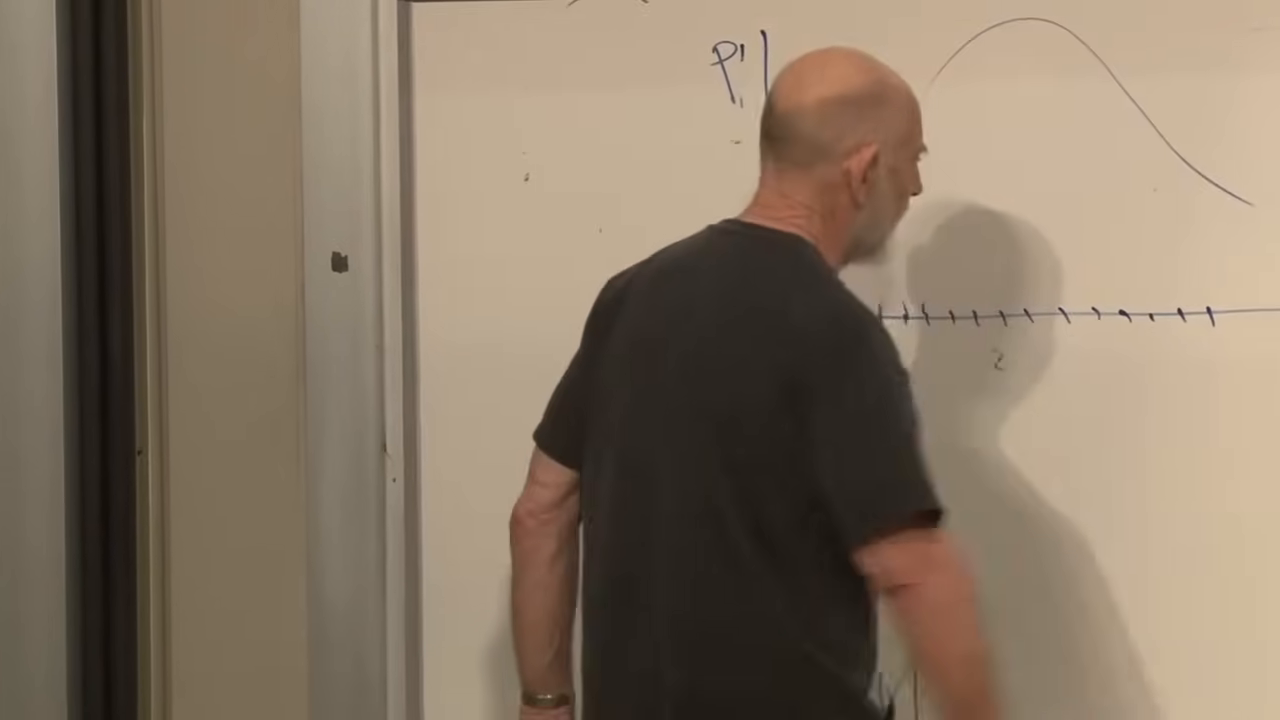
\includegraphics[width=0.92\textwidth]{lecture_01_figure_05.png}\caption{Eine Wahrscheinlichkeitsverteilung über diskreten Zustandsbezeichnungen. Für die Entropie ist die Breite der Verteilung entscheidend, nicht der genaue Kurvenverlauf.}\lectureframe{01:14:40}\end{figure}

\begin{figure}[htbp]\centering
\resizebox{\linewidth}{!}{%
\begin{tikzpicture}[>=Latex,scale=0.93]
\draw[->] (-4.2,0) -- (4.4,0) node[right] {state label \(i\)};
\draw[->] (-4,0) -- (-4,3.2) node[above] {$p_i$};
\foreach \x in {-3.6,-3.1,...,3.6}
  \draw (\x,0.08) -- (\x,-0.08);
\draw[very thick]
  plot[smooth] coordinates {
  (-3.7,0.12) (-3.0,0.28) (-2.3,0.72) (-1.6,1.45)
  (-0.9,2.25) (-0.2,2.65) (0.5,2.28) (1.2,1.55)
  (1.9,0.88) (2.7,0.38) (3.5,0.14)};
\draw (-1.8,-0.18) -- (-1.8,-0.5);
\draw (1.8,-0.18) -- (1.8,-0.5);
\draw[<->] (-1.8,-0.46) -- (1.8,-0.46);
\node at (0,-0.82) {effective spread};
\end{tikzpicture}}\caption{Eine schmale Verteilung bedeutet weniger Ungewissheit als eine breite. Die Entropie muss die Verteilung als Ganzes erfassen.}\label{fig:sm1-probability-spread}\end{figure}

Die allgemeine Definition lautet
\begin{equation}
 S=-\sum_i p_i\log p_i.
 \label{eq:sm1-shannon-entropy}
\end{equation}
Mit \eqref{eq:sm1-expectation} ergibt sich
\begin{equation}
 S=-\langle\log p\rangle.
\end{equation}
Das Minuszeichen gleicht aus, dass \(\log p_i<0\) gilt, wenn \(0<p_i<1\) gilt.

\subsection{Wiedergewinnung des Ergebnisses für die Gleichverteilung}

Wir müssen prüfen, ob die allgemeine Formel die erste Definition reproduziert.
Für einen unbesetzten Zustand gilt \(p_i=0\), während \(\log p_i\) divergiert. Das Produkt
hat den wohldefinierten Grenzwert
\begin{equation}
 \lim_{p\to0^+}p\log p=0.
 \label{eq:sm1-plogp-limit}
\end{equation}
Zustände mit Wahrscheinlichkeit null tragen also nichts bei.

\begin{classroomqa}
\audiencequestion{Wenn \(p_i=0\) gilt, verschwindet der Term dann wirklich? Der Logarithmus
von null ist minus unendlich.}
\lecturerresponse{Der Term wird durch den Grenzwert
\(\lim_{p\to0^+}p\log p\) definiert, der null ist. Der Faktor \(p\) geht schneller gegen null,
als der Logarithmus divergiert. Daher leisten beliebig unwahrscheinliche Zustände
beliebig kleine Beiträge, und ein exakt unmöglicher Zustand trägt nichts bei.
\lecturetimestamp{01:18:27--01:19:46}}
\end{classroomqa}

Für jeden der \(M\) besetzten Zustände gilt \(p_i=1/M\). Daher
\begin{align}
 S
 &=-\sum_{\mathrm{occupied}\ i}
 \frac1M\log\!\left(\frac1M\right)\\
 &=-M\frac1M\log\!\left(\frac1M\right)\\
 &=-\log\!\left(\frac1M\right)
 =\log M.
 \label{eq:sm1-entropy-check}
\end{align}
Der allgemeine Ausdruck stimmt exakt mit dem Spezialfall überein. Eine breitere
Verteilung gewichtet mehr Alternativen merklich und hat deshalb eine größere
Entropie; eine schmalere Verteilung hat eine kleinere Entropie.

\begin{figure}[htbp]
\centering
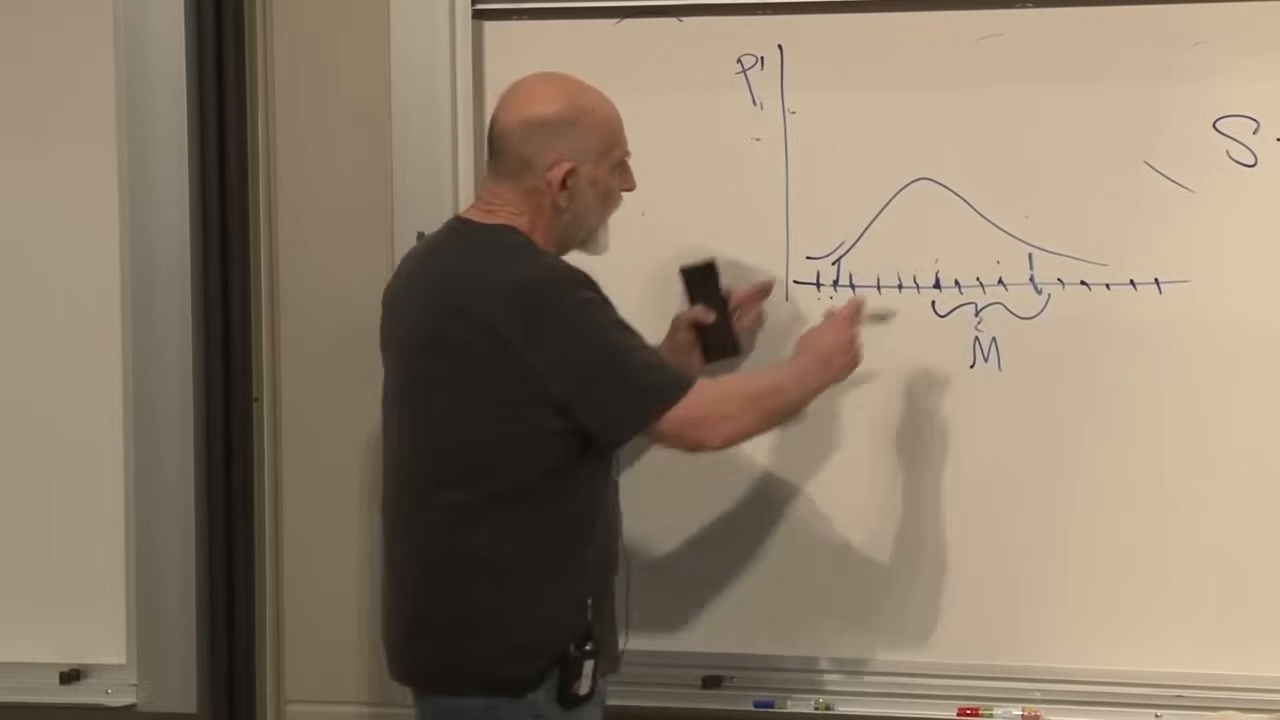
\includegraphics[width=0.92\textwidth]{lecture_01_figure_06.png}
\caption{Die markierte Breite \(M\) hebt den Zusammenhang zwischen der Streuung
der maßgeblichen Wahrscheinlichkeiten und der Entropie hervor.}
\lectureframe{01:16:42}
\end{figure}

Entropie ist einer Wahrscheinlichkeitsverteilung auf dem Zustandsraum zugeordnet. Sie ist
keine bloße Observable wie die Energie oder der Impuls eines einzelnen Mikrozustands. Ein exakter
Zustand lässt sich durch eine auf diesen Zustand konzentrierte Verteilung darstellen und
hat dann Entropie null; die Entropie ändert sich jedoch, wenn sich der Kenntnisstand
ändert.

\section{Münzen, Bits und explizites Abzählen}

Sei \(n\) die Anzahl der Münzen. Die Anzahl der mikroskopischen Konfigurationen ist
\begin{equation}
 N=2^n.
 \label{eq:sm1-coin-state-count}
\end{equation}
Wenn über die Münzen nichts bekannt ist, sind alle \(2^n\) Konfigurationen gleich
wahrscheinlich, und es gilt
\begin{equation}
 S_{\max}=\log(2^n)=n\log2.
 \label{eq:sm1-coin-max-entropy}
\end{equation}
Die Entropie ist additiv bezüglich der Anzahl unabhängiger Münzen.

Bei Logarithmen zur Basis \(2\) hat ein vollständig unbekanntes Zweizustandssystem
eine Entropie von einem Bit. Mit natürlichen Logarithmen beträgt sie \(\log2\). Die Einheit
ist Konvention; die zugrunde liegende Ordnung und Additivität bleiben unverändert.

Am anderen Extrem gilt: Wenn jede Münze bekannt ist, hat genau eine Konfiguration
die Wahrscheinlichkeit eins:
\begin{equation}
 S=0.
\end{equation}
Mehr Wissen bedeutet weniger Entropie.

Nehmen wir nun an, dass genau eine der \(n\) Münzen Zahl zeigt, alle übrigen Kopf,
und die Position der Münze mit Zahl unbekannt ist. Es gibt \(n\) gleich wahrscheinliche
Konfigurationen, eine für jede mögliche Position dieser Münze, also gilt
\begin{equation}
 S=\log n.
 \label{eq:sm1-one-tail-entropy}
\end{equation}
Dies ist im Allgemeinen kein ganzzahliges Vielfaches von \(\log2\). Ein Bit ist eine praktische
Einheit und bedeutet nicht, dass jede Entropie nur in ganzen Bits auftreten kann.

\begin{classroomqa}
\audiencequestion{Tritt \(\log2\) nur deshalb auf, weil jede Münze zwei
mögliche Zustände hat? Ergäbe ein Element mit drei Zuständen \(\log3\)?}
\lecturerresponse{Genau. Ein vollständig unbekanntes Element mit \(k\) möglichen
Zuständen trägt \(\log k\) bei. Binäre Schalter sind in Computern besonders praktisch,
weil physische Schalter sich auf natürliche Weise in zwei stabile Zustände bringen lassen
und weil zwei die kleinste nichttriviale ganze Zahl ist.
\lecturetimestamp{01:29:55--01:30:48}}
\end{classroomqa}

\begin{classroomqa}
\audiencequestion{Welche Basis ist für den Logarithmus gemeint?}
\lecturerresponse{In diesen physikalischen Formeln bezeichnet \(\log\) den natürlichen
Logarithmus. Informationstheoretiker verwenden häufig die Basis \(2\), sodass die Entropie
direkt in Bits gemessen wird. Ein Wechsel der Basis multipliziert jede Entropie mit demselben
Umrechnungsfaktor und ändert keine physikalische Schlussfolgerung.
\lecturetimestamp{01:30:49--01:32:06}}
\end{classroomqa}

\section{Entropie im kontinuierlichen Phasenraum}

Kehren wir zu einem klassischen Phasenraum \(\Gamma\) zurück. Ist die Wahrscheinlichkeitsdichte
in einem Gebiet mit Volumen \(V_\Gamma\) gleichförmig und außerhalb davon null, so lautet das
Analogon zum Abzählen von \(M\) gleich wahrscheinlichen Zuständen
\begin{equation}
 S=\log\!\left(\frac{V_\Gamma}{V_0}\right).
 \label{eq:sm1-continuous-uniform}
\end{equation}
Dabei ist \(V_\Gamma\) das Volumen im vollständigen hochdimensionalen Raum der Koordinaten
und Impulse, nicht das gewöhnliche räumliche Volumen. Das feste Volumen \(V_0\) ist eine
Referenzzelle im Phasenraum, durch die der Logarithmus dimensionslos wird. Setzt man
\(V_0=1\), erhält man die an der Tafel verwendete Kurzform \(S=\log V_\Gamma\).

Für eine allgemeine Wahrscheinlichkeitsdichte \(P(q,p)\) wird die diskrete Summe durch ein
Phasenraumintegral ersetzt. Die Normierung lautet
\begin{equation}
 \int_\Gamma d\Gamma\,P(q,p)=1,
 \label{eq:sm1-continuous-normalization}
\end{equation}
und die Entropie ist
\begin{equation}
 S=-\int_\Gamma d\Gamma\,
 P(q,p)\log\!\bigl[P(q,p)V_0\bigr].
 \label{eq:sm1-continuous-entropy}
\end{equation}
Die Dichte ist die Wahrscheinlichkeit pro Phasenraumzelle. Begrifflich misst
\eqref{eq:sm1-continuous-entropy} weiterhin, wie breit die Wahrscheinlichkeit
verteilt ist; für einen gleichförmigen Fleck ergibt sich daraus der Logarithmus des
besetzten Volumens, gemessen in Einheiten der Referenzzelle. Eine Änderung dieser festen
Zelle verschiebt jede kontinuierliche Entropie um dieselbe additive Konstante und lässt
Entropiedifferenzen unverändert.

\begin{classroomqa}
\audiencequestion{Warum hat sich das Koordinatensymbol von \(x\) zu \(q\) geändert?}
\lecturerresponse{Physikalisch ändert sich dadurch nichts. In der klassischen Mechanik
verwendet man für Koordinaten häufig entweder \(x\) oder \(q\) und für konjugierte Impulse
\(p\). Der Wechsel der Notation war lediglich ein Versehen; die Konstruktion des Phasenraums
ist dieselbe.
\lecturetimestamp{01:37:10--01:37:39}}
\end{classroomqa}

Temperatur und die Boltzmann-Verteilung werden bewusst auf später verschoben. Als Nächstes
werden wir das thermische Gleichgewicht definieren und anschließend seine
Wahrscheinlichkeitsverteilung bestimmen.

\section{Fragen zu Korrelation, Additivität und Information}

\subsection{Korrelation bedeutet, dass eine Messung die Verteilung einer anderen Größe verändert}

Bei vollständiger Unkenntnis über unabhängige Münzen wird jeder Konfiguration dieselbe
Wahrscheinlichkeit zugewiesen. Eine Messung an einer Münze verrät dann nichts über irgendeine
andere Münze. Deren Verteilungen bleiben unverändert.

Das Ensemble mit genau einer Münze, die Zahl zeigt, ist anders. Misst man bei einer Münze Zahl,
zeigt jede andere mit Sicherheit Kopf. Zeigt die gemessene Münze Kopf, muss die einzige Münze mit Zahl
unter den verbleibenden \(n-1\) Münzen sein; daher hat jede verbleibende Position die bedingte Wahrscheinlichkeit
\begin{equation}
\begin{aligned}
 p(&\text{tail at a specified remaining position}\\
   &\mid\text{measured head})=\frac{1}{n-1}.
\end{aligned}
 \label{eq:sm1-conditional-tail}
\end{equation}
Das ist Korrelation: Wenn man eine Variable kennt, ändert sich die der anderen zugewiesene
Wahrscheinlichkeitsverteilung.

\begin{classroomqa}
\audiencequestion{Wurde in den Entropiebeispielen Unabhängigkeit der Münzen vorausgesetzt?}
\lecturerresponse{Nur wenn vollständige Unkenntnis durch gleiche
Wahrscheinlichkeiten für alle \(2^n\) Konfigurationen dargestellt wurde. In diesem Fall lässt eine Messung an einer
Münze die Verteilungen der übrigen unverändert. Das Beispiel mit genau einer Münze, die Zahl zeigt,
ist ausdrücklich korreliert: Eine Messung aktualisiert, was an anderer Stelle möglich ist.
Die angegebene Information bestimmt, welche Wahrscheinlichkeitsverteilung verwendet wird.
\lecturetimestamp{01:38:43--01:41:58}}
\end{classroomqa}

Das Beispiel mit den getrennten Zyklen hat dieselbe logische Struktur. Eine Messung des erhaltenen
Labels \(+1\) oder \(-1\) beschränkt alle späteren Zustände auf einen Sektor.
Die Konditionierung auf erhaltene Information ändert die zulässige Verteilung.

Für unkorrelierte Systeme ist die Entropie additiv. Wenn
\begin{equation}
 p_{ij}=p_i^{(A)}p_j^{(B)},
\end{equation}
Dann gilt
\begin{align}
 S_{AB}
 &=-\sum_{i,j}p_i^{(A)}p_j^{(B)}
 \log\!\left[p_i^{(A)}p_j^{(B)}\right]\\
 &=S_A+S_B.
 \label{eq:sm1-entropy-additivity}
\end{align}
Korrelationen verhindern diese Faktorisierung und verringern die unabhängige
Ungewissheit des Paars.

Stell dir als Übung eine Reihe binärer Variablen vor, bei der ein Element im Zustand „oben“ dazu führt,
dass jeder Nachbar mit Wahrscheinlichkeit drei Viertel im Zustand „unten“ ist. Eine Messung an einem Ort
ändert unmittelbar, was über nahegelegene Orte bekannt ist. Eine solche Verteilung ist korreliert, und ihre
Entropie lässt sich nicht durch Addition isolierter Ein-Ort-Entropien bestimmen, ohne diese Korrelationen
zu berücksichtigen.

\subsection{Boltzmann, Shannon und die quantenmechanische Unbestimmtheit}

\begin{classroomqa}
\audiencequestion{Wie hängt die ältere thermodynamische Entropie mit der
informationstheoretischen Entropie von Shannon zusammen?}
\lecturerresponse{In beiden Fällen tritt dieselbe Funktionalform auf:
\(-\sum_i p_i\log p_i\). Shannon verwendete häufig die Basis \(2\), während Physiker
üblicherweise natürliche Logarithmen verwenden und die Boltzmann-Konstante wieder einsetzen,
wenn die Entropie in thermodynamischen Einheiten angegeben wird. Der mathematische Unterschied
besteht nur in einem festen Umrechnungsfaktor, auch wenn die physikalischen Fragen, aus denen
die Wahrscheinlichkeiten hervorgehen, sehr verschieden sein können.
\lecturetimestamp{01:44:05--01:46:06}}
\end{classroomqa}

Für gleich wahrscheinliche Mikrozustände schreibt man die thermodynamische Formel oft als
\begin{equation}
 S_{\mathrm{thermo}}=k_{\mathrm B}\log W,
 \label{eq:sm1-boltzmann-formula}
\end{equation}
Dabei ist \(W\) die Anzahl der zugänglichen Mikrozustände. In Einheiten mit
\(k_{\mathrm B}=1\) ist dies genau \(S=\log W\). Die Boltzmann-Konstante rechnet zwischen Temperatureinheiten
und Energieeinheiten um; die natürliche mikroskopische Skala der Temperatur ist die Energie.

\begin{classroomqa}
\audiencequestion{Ist diese Entropie einfach eine andere Form der Heisenbergschen
Unschärferelation?}
\lecturerresponse{Nein. Die hier betrachtete Entropie misst die Ungewissheit einer
Wahrscheinlichkeitsverteilung über mögliche Zustände. In der Quantensprache ist sie die
Ungewissheit eines gemischten Zustands, nicht die intrinsische Messunsicherheit, die auch
bei einem reinen Zustand bestehen bleiben kann. Diese beiden Begriffe müssen klar
auseinandergehalten werden.
\lecturetimestamp{01:46:07--01:47:31}}
\end{classroomqa}

\section{Was bisher gezeigt wurde}

Ausgangspunkt war nicht eine Zufälligkeit der Gesetze. Eine deterministische Dynamik erzeugt
zusammen mit unvollständiger Kenntnis des Anfangszustands bereits Wahrscheinlichkeiten. Eine einzelne
Bahn weist Zuständen Gewichte zu, je nachdem, wie viel Zeit in jedem Zustand verbracht wird; getrennte
Bahnen machen Erhaltungsgrößen sichtbar und erfordern vorherige Gewichte für die verschiedenen
Sektoren. Zulässige mikroskopische Gesetze bewahren Unterscheidungen. In einem endlichen Zustandsraum
bedeutet das, dass an jedem Zustand genau ein Pfeil ankommt und einer abgeht; in der kontinuierlichen
Mechanik entspricht dem das Liouville-Theorem.

Diese Struktur führt zunächst zu
\begin{equation}
 S=\log M
\end{equation}
für \(M\) gleich wahrscheinliche besetzte Zustände, dann zu
\begin{equation}
 S=-\sum_i p_i\log p_i,
\end{equation}
und schließlich zu seinem Phasenraumintegral. Entropie beschreibt eine Wahrscheinlichkeitsverteilung
und damit einen Kenntnisstand. Die feinkörnige Information bleibt durch das mikroskopische Gesetz
erhalten, selbst wenn eine praktische grobkörnige Beschreibung sie nicht mehr nachverfolgt.

Die Energieerhaltung liefert den ersten Hauptsatz, während die Additivität der Teilenergien eine
vernachlässigbare Wechselwirkungsenergie voraussetzt. Für die Entropie gilt eine entsprechende
Bedingung: Die Wahrscheinlichkeiten der Teilsysteme müssen unkorreliert sein. Diese beiden Arten
von Additivität bereiten den nächsten Schritt vor, bei dem thermisches Gleichgewicht, Temperatur
und die Boltzmann-Verteilung Energie mit Wahrscheinlichkeit verknüpfen.
